\documentclass{article}
\usepackage{graphicx} % Required for inserting images

\usepackage[utf8]{inputenc}
\usepackage[T5]{fontenc}
\usepackage[vietnamese]{babel}       % Required for Vietnamese

\usepackage{booktabs} 
\usepackage{listings}
\usepackage{xcolor}
\usepackage{subcaption}

\definecolor{codebg}{rgb}{0.95,0.95,0.95} % Màu nền nhẹ

\lstset{
    language=Python, % Ngôn ngữ mã nguồn (Python, C, Java, etc.)
    basicstyle=\ttfamily\footnotesize, % Font chữ
    backgroundcolor=\color{codebg}, % Màu nền
    frame=single, % Viền xung quanh khung code
    numbers=left, % Đánh số dòng
    numberstyle=\tiny\color{gray}, % Màu số dòng
    keywordstyle=\color{blue}, % Màu từ khóa (if, else, while, etc.)
    stringstyle=\color{red}, % Màu chuỗi (chữ trong dấu "")
    commentstyle=\color{orange}, % Màu chú thích
    tabsize=4, % Kích thước tab
    breaklines=true, % Xuống dòng nếu quá dài
}
\addto\captionsvietnamese{\renewcommand{\figurename}{Fig.}}
\addto\captionsvietnamese{\renewcommand{\tablename}{Table}}
\usepackage{graphicx}
\usepackage[paperheight=6in,
   paperwidth=5in,
   top=10mm,
   bottom=20mm,
   left=10mm,
   right=10mm]{geometry}

\title{DSA}
\author{Tôn Huỳnh Chí}
\date{March 2025}

\begin{document}
\maketitle

\section{Introduction} 

The R-tree was proposed by Guttman in 1984, and aimed at handling geometrical data, such as points, line segments, surfaces, volumes, and hypervolumes in high-dimensional spaces. \par
R-trees are hierarchical data structures based on B+ trees \textit{(self-balancing tree data structure used in databases and file systems for efficient indexing and range searches)}. They are used for the dynamic organization of a set of d-dimensional geometric objects representing them by the minimum bounding d-dimensional rectangles \textit{(MBRs)}. Each node of the R-tree corresponds to the MBR that bounds its children. The leaves of the tree contain pointers to the database objects instead of pointers to children nodes.\par
It must be noted that the MBRs that surround different nodes may overlap each other. Besides, an MBR can be included \textit{(in the geometrical sense)} in many nodes, but it can be associated to only one of them. This means that a spatial search may visit many nodes before confirming the existence of a given MBR. Also, it is easy to see that the representation of geometric objects through their MBRs may result in false alarms. To resolve false alarms, the candidate objects must be examined. For instance, Figure 1 illustrates the case where two polygons do not intersect each other, but their MBRs do. Therefore, the R-tree plays the role of a filtering mechanism to reduce the costly direct examination of geometric objects.

\begin{figure}[h]
\centering
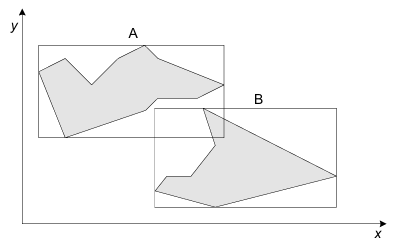
\includegraphics[width=0.5\textwidth]{1.1.png}
\caption{\textit{An example of intersecting MBRs, where the polygons do not intersect.}}
\label{fig:1.1}
\end{figure}


\section{Structure}

An R-tree of order (m,M) has the following characteristics:
\begin{itemize}
    \item Each leaf node (unless it is the root) can host up to M entries, whereas the minimum allowed number of entries is m $\leq$  M/2. Each entry is of the form (mbr,oid), such that mbr is the MBR that spatially contains the object and oid is the object’s identifier.
    \item The number of entries that each internal node can store is again between m $\leq$ M/2 and M. Each entry is of the form (mbr,p), where p is a pointer to a child of the node and mbr is the MBR that spatially contains the MBRs contained in this child.
    \item The minimum allowed number of entries in the root node is 2, unless it is a leaf (in this case, it may contain zero or a single entry).
\end{itemize}

From the definition of the R-tree, it follows that it is a \textbf{height-balanced tree}.
As mentioned, it comprises a generalization of the B+-tree structure for many
dimensions. R-trees are \textbf{dynamic data structures}, i.e., global reorganization is
not required to handle insertions or deletions.

Figure 2 show a set of the MBRs of some data geometric objects.\par

\begin{figure}[h]
\centering
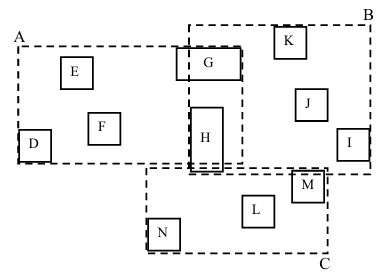
\includegraphics[width=0.5\textwidth]{1.2.png}
\caption{\textit{A, B, C is the MBRs of internal nodes, the others are the MBRs of the data objects.}}
\label{fig:1.2}
\end{figure}

Figure 3 show the R-tree that corresponds to the MBRs of Figure 2. The root node contains the MBRs of the internal nodes A, B, and C. The MBRs of the data objects are stored in the leaves of the tree. 

\begin{figure}[h]
\centering
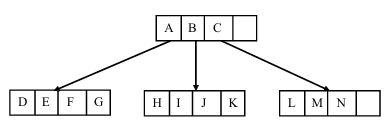
\includegraphics[width=0.5\textwidth]{1.3.png}
\caption{\textit{An R-tree that corresponds to the MBRs of Figure 2.}}
\label{fig:1.3}
\end{figure}

Let an R-tree store N data rectangles. In this case the maximum value for its height h is: $h_{max} = \lceil \log_2 N \rceil - 1$ \par
The maximum number of nodes can be derived by summing the maximum
possible number of nodes per level.
This number comes up when all nodes contain the minimum allowed number of entries, i.e., m. 
Therefore, it results
that the maximum number of nodes in an R-tree is equal to: $\sum_{i=1}^{h_{max}} \lceil N / m^i \rceil = \lceil N / m \rceil + \lceil N / m^1 \rceil + \lceil N / m^2 \rceil + \dots + 1$\par

\begin{table}[h]
    \centering
    \begin{tabular}{lcr}
        \toprule
        Root & Internal nodes & Leaf nodes \\
        \midrule
        min entries is 2 & min entries is m & min entries is m \\
        unless it is a leaf & max entries is M & max entries is M \\
        \midrule
        & data to child nodes & data objects \\
        \midrule
        \multicolumn{3}{c}{Hieght-balanced tree} \\
        \multicolumn{3}{c}{$h_{max} = \lceil \log_2 N \rceil - 1$} \\
        \multicolumn{3}{c}{$NumNode_{max} = \sum_{i=1}^{h_{max}} \lceil N / m^i \rceil$}\\
        \bottomrule
    \end{tabular}
    \caption{\textit{R-tree characteristics}}
\end{table}


\section{Operations}

\subsection{Search}
\textbf{Problem:} Find all data rectangles that are intersected by Q. This is denoted as a range (or window) query.\\
\textit{For a node entry E, E.mbr denotes the corresponding MBR, and E.p is the corresponding pointer to the next level. If the node is a leaf, then E.p denotes the corresponding object identifier (oid).}
\lstinputlisting[language=C++]{search.cpp}

\par 
Below is the example of the search operation. Red lines rectangle is the query rectangle, green lines rectangle is the MBR of the current node, and blue one is the answer.\\
\begin{figure}[h]
\centering
    \begin{subfigure}{0.3\textwidth}
    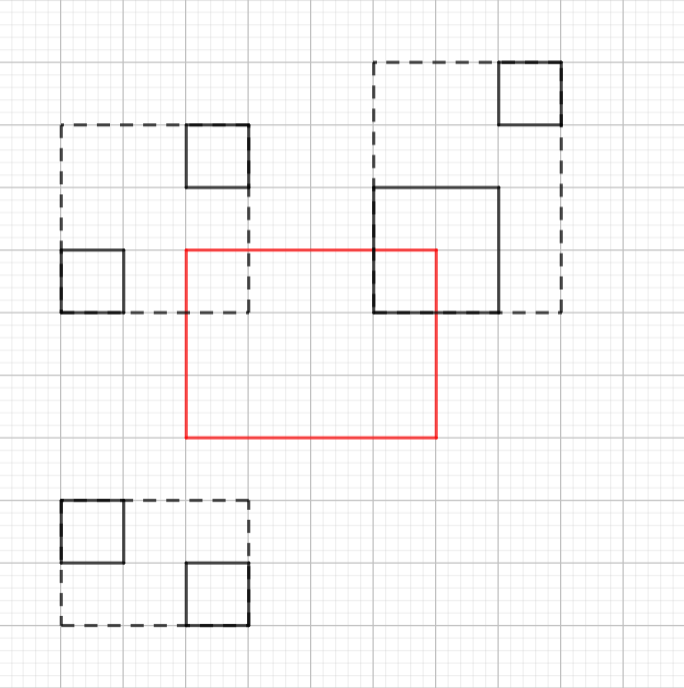
\includegraphics[width=\textwidth]{search/1.png}
    \caption{Step 1}
    \centering
    \end{subfigure}
    \begin{subfigure}{0.3\textwidth}
    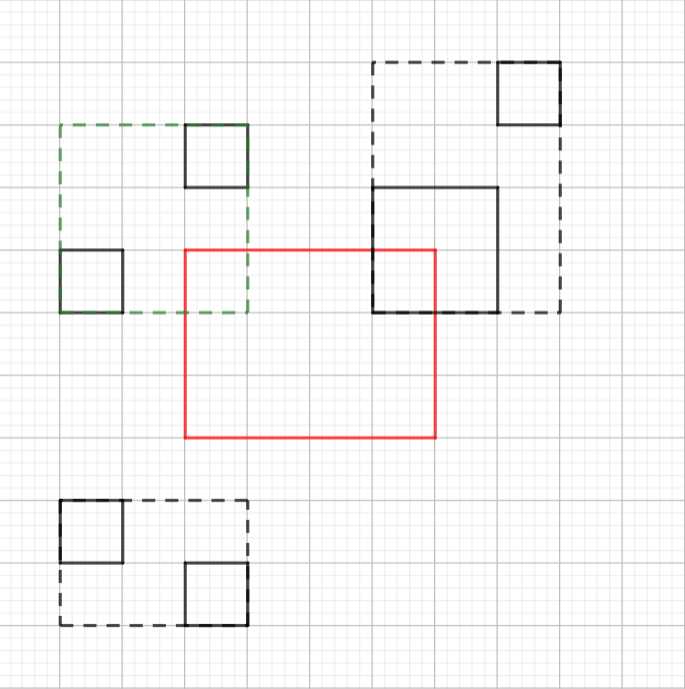
\includegraphics[width=\textwidth]{search/2.png}
    \caption{Step 2}
    \centering
    \end{subfigure}
    \begin{subfigure}{0.3\textwidth}
    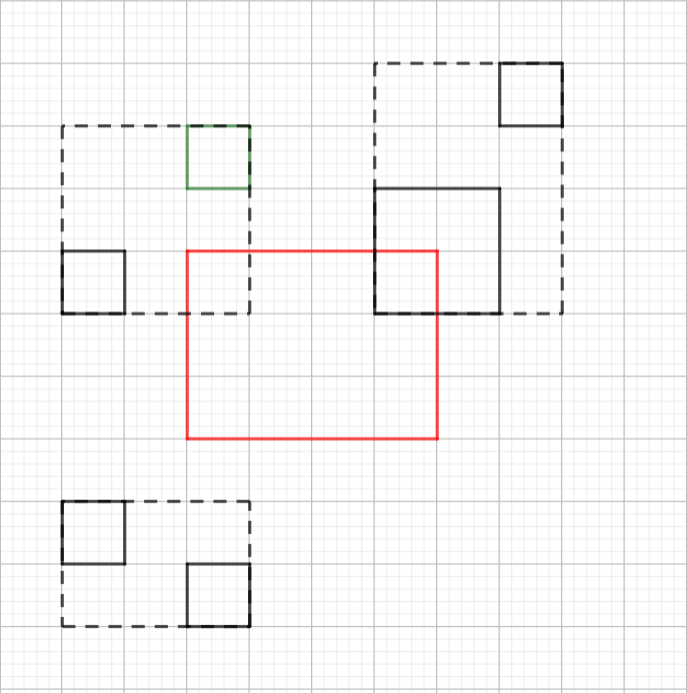
\includegraphics[width=\textwidth]{search/3.png}
    \caption{Step 3}
    \centering
    \end{subfigure}
    \begin{subfigure}{0.3\textwidth}
    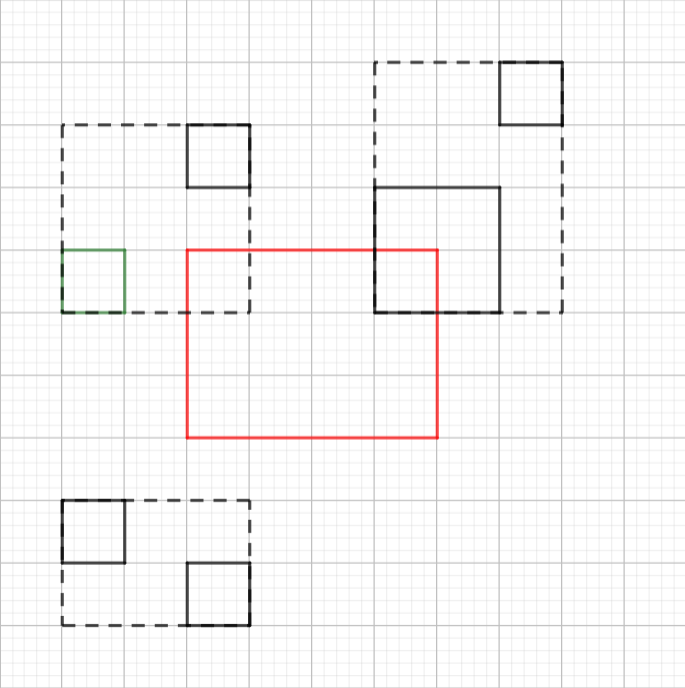
\includegraphics[width=\textwidth]{search/4.png}
    \caption{Step 4}
    \centering
    \end{subfigure}
    \begin{subfigure}{0.3\textwidth}
    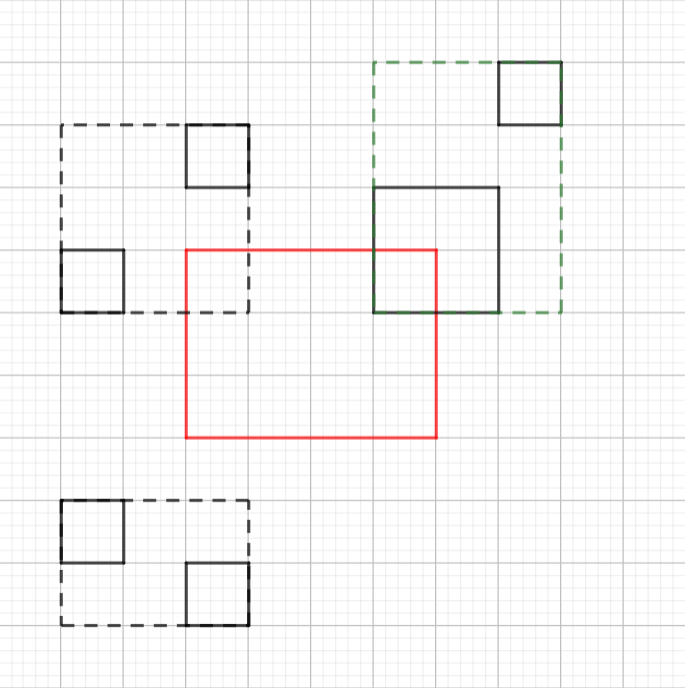
\includegraphics[width=\textwidth]{search/5.png}
    \caption{Step 5}
    \centering
    \end{subfigure}
    \begin{subfigure}{0.3\textwidth}
    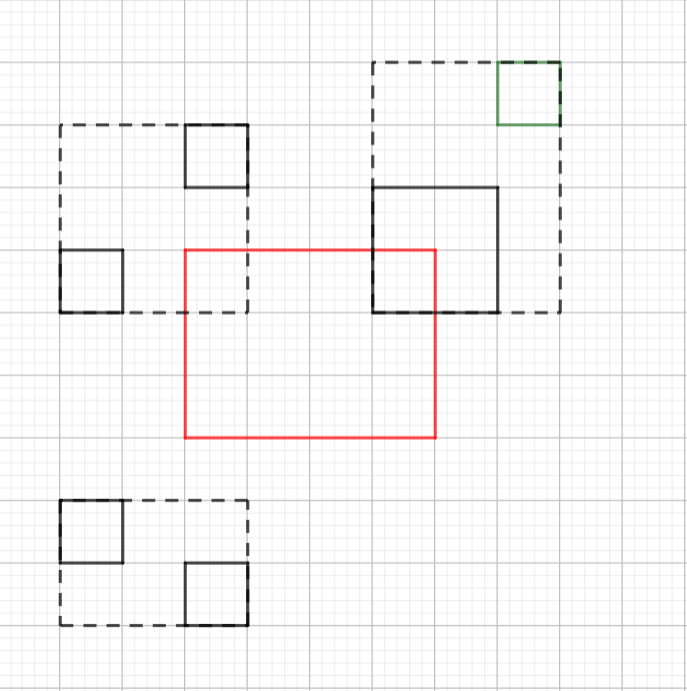
\includegraphics[width=\textwidth]{search/6.png}
    \caption{Step 6}
    \centering
    \end{subfigure}
    \begin{subfigure}{0.3\textwidth}
    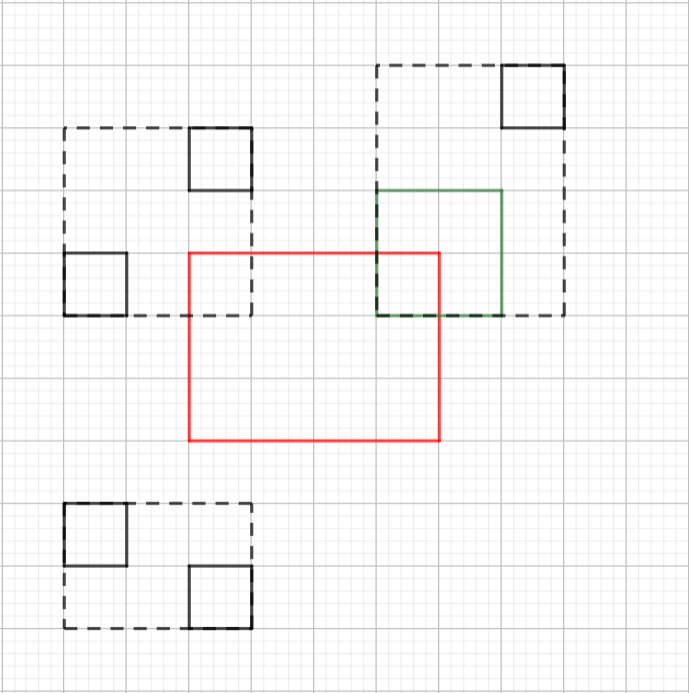
\includegraphics[width=\textwidth]{search/7.png}
    \caption{Step 7}
    \centering
    \end{subfigure}
    \begin{subfigure}{0.3\textwidth}
    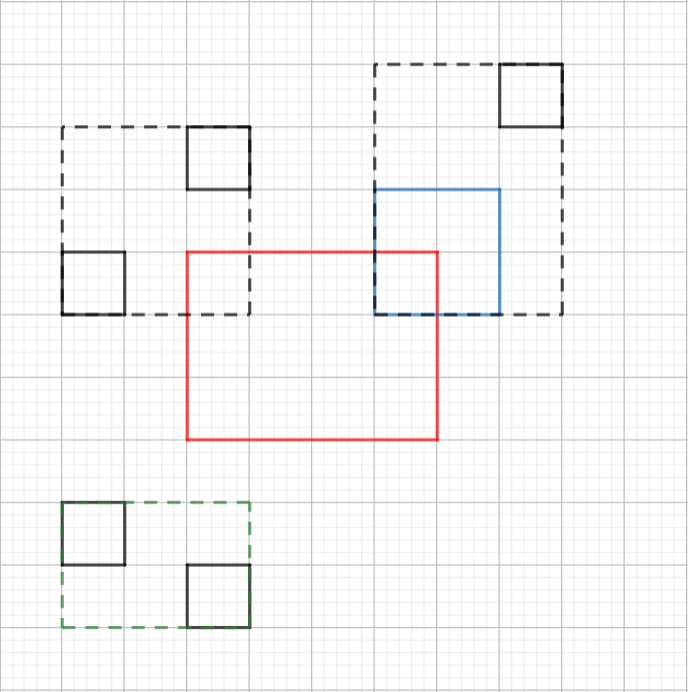
\includegraphics[width=\textwidth]{search/8.png}
    \caption{Step 8}
    \centering
    \end{subfigure}
    \begin{subfigure}{0.3\textwidth}
    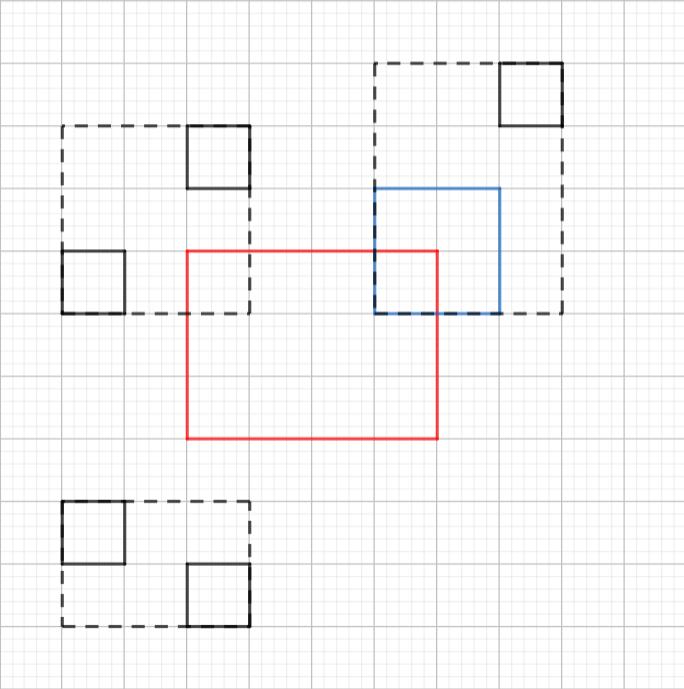
\includegraphics[width=\textwidth]{search/9.png}
    \caption{Step 9}
    \centering
    \end{subfigure}
\caption{\textit{Search operation}}

\end{figure} 
\clearpage

\subsection{Insertion}

\textbf{Problem:} Insert a new data rectangle R into the R-tree.\\
\textbf{Concept:} The R-tree is traversed to locate an appropriate leaf to accommodate the new entry. The entry is inserted in the found leaf and, then all nodes within the path from the root to that leaf are updated accordingly. In case the found leaf cannot accommodate the new entry because it is full \textit{(it already contains M entries)}, then it is split into two nodes.

\lstinputlisting[language=C++]{insert.cpp}

\textbf{Split - goal:} 

\begin{itemize}
    \item The leaf node has M entries, and one new entry to be inserted, how to partition the M+1 mbrs into two nodes, such that:
    \begin{itemize}
        \item The total area of the two nodes is minimized
        \item The overlapping of the two nodes is minimized
    \end{itemize}
    \item Sometimes the two goals are conflicting: Using 1 as the primary goal
\end{itemize}

There are three alternatives to handle splits that were proposed by Guttman.

\begin{itemize}
    \item \textbf{Linear split:} Choose two objects as seeds for the two nodes, where these objects are as far apart as possible. Then consider each remaining object in a random order and assign it to the node requiring the smallest enlargement of its respective MBR.\\
    For example with some 2-D objects:
    \begin{table}[h]
        \centering
        \begin{tabular}{|c|c|c|}
            \hline
            MBRs & bottom left & top right \\
            \hline
            A & (1, 1) & (3, 4) \\
            B & (2, 3) & (5, 6) \\
            C & (6, 2) & (8, 5) \\
            D & (7, 6) & (9, 9) \\
            E (new) & (4, 4) & (6, 7) \\
            \hline
        \end{tabular}
    \end{table}
    \\
    Use A and D as seeds
    \begin{table} [h]
        \centering
        \begin{tabular}{|c|c|c|c|}
            \hline
            MBRs & MBR if added to A & MBR if added to D & Assigned to \\
            \hline
            B & small increase & large increase & group A\\ 
            C & large increase & small increase & group D\\
            E & small increase & large increase & group A\\
            \hline
        \end{tabular}
    \end{table}
    \\
    \clearpage
    After the split
    \begin{table} [h]
        \centering
        \begin{tabular}{|c|c|}
            \hline
            Group & MBRs \\
            \hline
            A & (1, 1), (4, 4), (6, 7) \\
            \hline
            D & (7, 6), (9, 9) \\
            \hline
        \end{tabular}
    \end{table}
    \item \textbf{Quadratic split:} Choose two objects as seeds for the two nodes, where these objects if put together create as much dead space as possible \textit{(dead space is the space that remains from the MBR if the areas of the two objects are ignored)}. 
    Then, until there are no remaining objects, insert the object $e$ such that $e$ expands a group with the minimum area, \textit {(if tie \textbf{Choose the group of small area} - \textbf {Choose the group of fewer elements)}}.\\
    For example with some 2-D objects:
    \begin{table}[h]
        \centering
        \begin{tabular}{|c|c|c|}
            \hline
            MBRs & bottom left & top right \\
            \hline
            A & (1, 1) & (3, 4) \\
            B & (2, 3) & (5, 6) \\
            C & (6, 2) & (8, 5) \\
            D & (7, 6) & (9, 9) \\
            E (new) & (4, 4) & (6, 7) \\
            \hline
        \end{tabular}
    \end{table}
    \\
    \clearpage
    Calculate the dead space
    \begin{table} [h]
        \centering
        \begin{tabular}{|c|c|c|c|c|}
            \hline 
            Pair & Resulting MBR & Area & intersection area & Wasted area \\
            \hline
            A, B & (1, 1), (5, 6) & 20 & 1 & 14\\
            \hline
            A, C & (1, 1), (8, 5) & 28 & 0 & 16\\
            \hline
            A, D & (1, 1), (9, 9) & 64 & 0 & 52(worst)\\
            \hline
            A, E & (1, 1), (6, 7) & 30 & 0 & 18\\
            \hline
            B, C & (2, 2), (8, 6) & 24 & 0 & 9\\
            \hline
            B, D & (2, 3), (9, 9) & 42 & 0 & 27\\
            \hline
            B, E & (2, 3), (6, 7) & 16 & 2 & 3\\
            \hline
            C, D & (6, 2), (9, 9) & 21 & 0 & 9\\
            \hline
            C, E & (4, 2), (8, 7) & 20 & 0 & 8\\
            \hline
            D, E & (4, 6), (9, 9) & 25 & 0 & 13\\
            \hline
        \end{tabular}
    \end{table}
    \\
    Use A and D as seeds
    \lstinputlisting[language=c++]{qudratic.py}

    \item \textbf{Exponential split:} All possible groupings are exhaustively tested and the best is chosen with respect to the minimization of the MBR enlargement.
\end{itemize}

\clearpage

Illustrate for insert operation, in 2-d space:

\begin{figure}[h]
    \centering
        \begin{subfigure}{0.3\textwidth}
        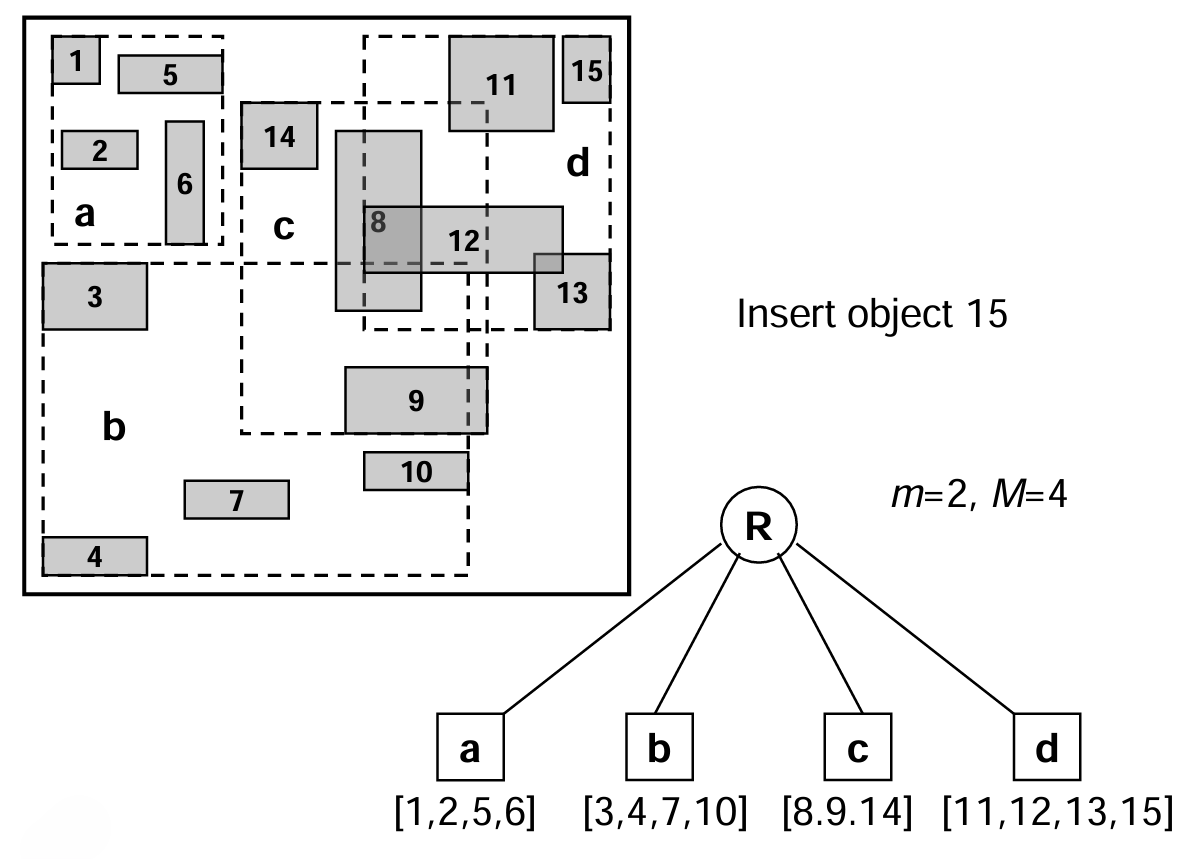
\includegraphics[width=\textwidth]{insert1 (1).png}
        \caption{Step 1}
        \centering
        \end{subfigure}
        \begin{subfigure}{0.3\textwidth}
        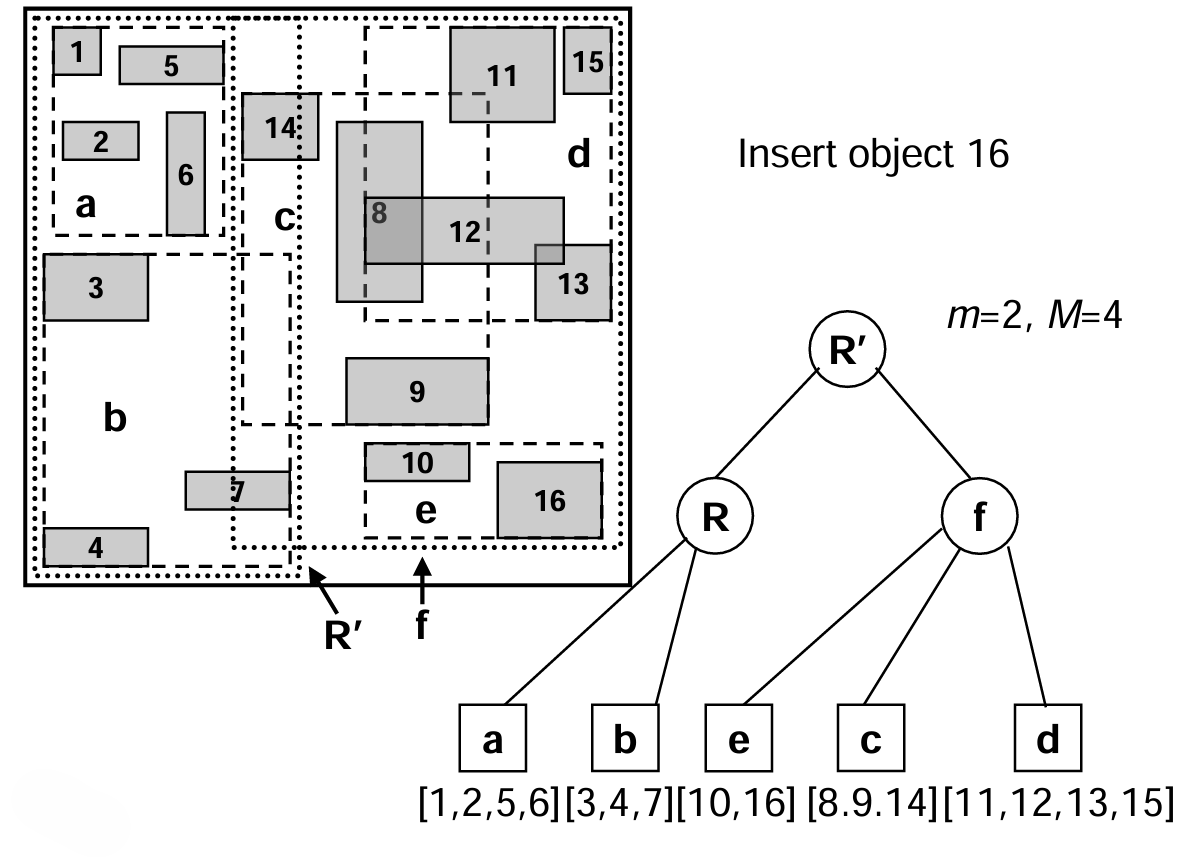
\includegraphics[width=\textwidth]{insert1 (2).png}
        \caption{Step 2}
        \centering
        \end{subfigure}
    \caption{\textit{Insert operation}}
\end{figure}

\subsection{Deletion}


\end{document}